% THIS IS SIGPROC-SP.TEX - VERSION 3.1
% WORKS WITH V3.2SP OF ACM_PROC_ARTICLE-SP.CLS
% APRIL 2009
%
% It is an example file showing how to use the 'acm_proc_article-sp.cls' V3.2SP
% LaTeX2e document class file for Conference Proceedings submissions.
% ----------------------------------------------------------------------------------------------------------------
% This .tex file (and associated .cls V3.2SP) *DOES NOT* produce:
%       1) The Permission Statement
%       2) The Conference (location) Info information
%       3) The Copyright Line with ACM data
%       4) Page numbering
% ---------------------------------------------------------------------------------------------------------------
% It is an example which *does* use the .bib file (from which the .bbl file
% is produced).
% REMEMBER HOWEVER: After having produced the .bbl file,
% and prior to final submission,
% you need to 'insert'  your .bbl file into your source .tex file so as to provide
% ONE 'self-contained' source file.
%
% Questions regarding SIGS should be sent to
% Adrienne Griscti ---> griscti@acm.org
%
% Questions/suggestions regarding the guidelines, .tex and .cls files, etc. to
% Gerald Murray ---> murray@hq.acm.org
%
% For tracking purposes - this is V3.1SP - APRIL 2009

\documentclass{acm_proc_article-sp}

\usepackage{amsmath}
\usepackage{caption}
\usepackage{float}
\usepackage{graphicx} % support the \includegraphics command and options
% for osx:
\usepackage[backend=biber]{biblatex}
%\usepackage{biblatex}
\usepackage{subcaption}

\renewcommand{\bibfont}{\footnotesize}
%\pagenumbering{gobble}
\usepackage{hyperref}
\addbibresource{report.bib}


\begin{document}

\title{Parallelised Pose Estimation for Automated Landing}
\subtitle{CS267: Project Report}
%
% You need the command \numberofauthors to handle the 'placement
% and alignment' of the authors beneath the title.
%
% For aesthetic reasons, we recommend 'three authors at a time'
% i.e. three 'name/affiliation blocks' be placed beneath the title.
%
% NOTE: You are NOT restricted in how many 'rows' of
% "name/affiliations" may appear. We just ask that you restrict
% the number of 'columns' to three.
%
% Because of the available 'opening page real-estate'
% we ask you to refrain from putting more than six authors
% (two rows with three columns) beneath the article title.
% More than six makes the first-page appear very cluttered indeed.
%
% Use the \alignauthor commands to handle the names
% and affiliations for an 'aesthetic maximum' of six authors.
% Add names, affiliations, addresses for
% the seventh etc. author(s) as the argument for the
% \additionalauthors command.
% These 'additional authors' will be output/set for you
% without further effort on your part as the last section in
% the body of your article BEFORE References or any Appendices.

\numberofauthors{3} %  in this sample file, there are a *total*
% of EIGHT authors. SIX appear on the 'first-page' (for formatting
% reasons) and the remaining two appear in the \additionalauthors section.
%
\author{
% You can go ahead and credit any number of authors here,
% e.g. one 'row of three' or two rows (consisting of one row of three
% and a second row of one, two or three).
%
% The command \alignauthor (no curly braces needed) should
% precede each author name, affiliation/snail-mail address and
% e-mail address. Additionally, tag each line of
% affiliation/address with \affaddr, and tag the
% e-mail address with \email.
%
% 1st. author
\alignauthor
Sunil Shah\\
       \email{sunil.shah@berkeley.edu}
% 2nd. author
\alignauthor
Nahush Bhanage\\
       \email{nahush@berkeley.edu}
% 3rd. author
\alignauthor 
Hoang Nguyen\\
       \email{hoanghw@berkeley.edu}
}

\date{12 May 2014}

\maketitle
\begin{abstract}
Current approaches for automated landing of unmanned aerial systems (UAS) are
based on GPS localization, which we show is quite inaccurate. We optimise a previously implemented computer vision based pose estimation algorithm to run in real time on a low cost open source embedded computer using open source software. .
\end{abstract}

%%%%%%%%%%%%%%%%%%%%%%%%%%%%%%%%%%%%%%%%%%%%%%%%%%%%%%%%%%%%%%%%%%%%%%%%%%%%%%
\section{Introduction}
The rise of the hobbyist unmanned aerial system movement has been driven by three factors: 1) the increasing availability and popularity of open source hardware and software, 2) the maker movement and 3) the availability of low cost sensors. These have led to communities such as DIYDrones, a message board where users developed the open source ArduPilot autopilot, initially based on the Arduino platform. In combination with such an autopilot, a user could feasibly 3D print (or purchase) their own multi-rotor frame, mount motors and wire to the autopilot radio control equipment used for ordinary radio control aircraft. For a total cost of approximately \$1,000, a user would have a fully autonomous aerial system.

 As the hobbyist UAS become more capable, an increasing number of researchers and startups are building products and systems using them.  Based on this trend, a federal mandate set in place in 2012 a requirement for the FAA to integrate unmanned aerial systems (UAS) into the national airspace by 2015 for civilian and commercial use.

General purpose open source hardware boards such as the Raspberry Pi or BeagleBone Black typically use the ARM processor architecture, a reduced instruction set computing (RISC) design. This is the architecture most commonly used in smartphones and allows users to run full Linux based operating system such as Ubuntu or Android onboard, with use of with standard libraries and utilities. (This is unlikely prototyping boards such as the Arduino which have their own special purpose environment which is user friendly but limited.) 

While increasing in computing power rapidly, RISC architectures lack the raw performance of more mature and advanced x86 processors which have the same or higher clock speeds but considerably more provisions for fast floating point operations, larger caches and increased processor level parallelism. However, the power, thermal efficiency and spatial gains from using a RISC architecture have made them compelling for power and payload constrained UAS.

In this project, we take a vision based pose estimation algorithm developed for a separate project and investigate parallel processing techniques to optimise its performance on a general purpose open source computer. Current methods of localisation for UAS rely upon GPS, which, unless augmented by additional ground stations transmitting from a known reference location, is inaccurate. In a test run of 10 automated landings where the UAS took off and attempted to land in the same location using GPS, we gained a mean accuracy of 195.33 cm \cite{berzanaccurate}.

Using a landing pad with a known design coupled with a webcam and computer on-board, it is possible to compute considerably accurate pose estimates using computer vision techniques \cite{berzanaccurate}. These permit the UAS to localise itself much more precisely than using GPS alone which enables precision hovering and landing. However, these computer vision techniques are computationally intensive, relying upon several passes over an image to extract features. In our earlier work, we were unable to get this operating at more than 3 frames a second on the BeagleBone Black embedded computer. 

The inner control loop of the ArduPilot autopilot software runs at 10 Hz - where it receives sensor data and outputs a control signal. This is deemed adequate for precise control of a UAS in all but the most extreme environmental conditions. Therefore, for pose estimation to be useful for UAS control, it is necessary to generate pose estimates at a rate of 10 Hz (or, 10 frames per second). Given that, in reality, certain frames are dropped due to motion blur, we strive for a rate of greater than 10 Hz.

We first survey prior work in section \ref{sec:prior-work}, then describe our system architecture in section \ref{sec:system-description}. In section \ref{sec:approach} we detail our approach to optimisation and in section \ref{sec:results} we show the results of this approach.

%%%%%%%%%%%%%%%%%%%%%%%%%%%%%%%%%%%%%%%%%%%%%%%%%%%%%%%%%%%%%%%%%%%%%%%%%%%%%%
\section{Prior Work\label{sec:prior-work}}
Our naive implementation was the result of a previous project and a full description of prior work related to automated landing approaches are available in that paper \cite{berzanaccurate}. The algorithm implemented is described by Sharp et al. in \cite{sharp_et_al_2001} and the overall approach is the same, although the exact implementation details may vary slightly. In their implementation, using highly optimised custom C code, they were able to each a frame rate of 30 frames per second. 

We consider other prior work related to high performance embedded computing. Several efforts have bene made to explore the effect of parallelising certain robotics appliations but these assume use of a desktop computer and often make use of general purpose computing on the GPU frameworks like CUDA or OpenCL. This doesn't translate well to the embedded computers due to the lack of vendor support for graphics chips that are provided. These chips often don't support heterogenous parallel programming languages, such as OpenCL or NVidia's CUDA. 

However, there are several efforts looking at optimising performance for ARM-based processors \cite{mitra2013use}. This is driven by growing smartphone usage, nearly all of which use ARM processor designs. Qualcomm, in particular, provides an ARM-optimised computer vision library for Android called FastCV. While this is optimised for their own series of processors, it does have generic ARM optimisations that are manufacturer agnostic. Efforts have been made to explore OpenCV optimisation for real-time computer vision applications too \cite{pulli2012real}.

A San Francisco based startup, Skycatch Inc., uses a BeagleBone Black to provide a custom runtime environment. This allows their users to write applications on top of their custom designed UAS in scripting language JavaScript. While the user friendliness of this approach is evident, it is also clear that using a high level interpreted application results in a tremendous loss of performance which makes it impossible to do all but the most basic of image processing in real-time. This implementation is also closed source. 

Other commercial entities, such as Cloud Cap Technologies, provide proprietary embedded computers running highly customised computer vision software. However, these cost many thousands of dollars and are difficult to \textit{hack}, making them impractical for research and startup use.

Ultimately, this project's contribution is to demonstrate the tools and techniques that can be used to implement highly performant vision algorithms onboard a UAS using low-cost open source hardware and open source software.

%%%%%%%%%%%%%%%%%%%%%%%%%%%%%%%%%%%%%%%%%%%%%%%%%%%%%%%%%%%%%%%%%%%%%%%%%%%%%%
\section{System Description\label{sec:system-description}}

\subsection{Hardware Architecture}
% Autopilot
% Embedded computer
% Peripheral hardware
% Architecture diagram

\subsection{Software Design}
% Operating system and library setup


\subsection{Automated Landing}

\subsubsection{Landing Pad Design}
\subsubsection{Algorithm Overview}
\paragraph{Corner Detection}
\paragraph{Pose Estimation}

\subsubsection{Real-time Control}

%%%%%%%%%%%%%%%%%%%%%%%%%%%%%%%%%%%%%%%%%%%%%%%%%%%%%%%%%%%%%%%%%%%%%%%%%%%%%%
\section{Approach\label{secapproach}}
% List of optimisations

\subsection{Profiling}



\subsection{Compiler Optimisations}
%% PARALLELISM HERE

\subsection{Library Optimisations}
%% PARALLELISM HERE

\subsection{Single-threaded Optimisations}

\subsection{Multi-threaded Optimisations}


%%%%%%%%%%%%%%%%%%%%%%%%%%%%%%%%%%%%%%%%%%%%%%%%%%%%%%%%%%%%%%%%%%%%%%%%%%%%%%
\section{Results\label{sec:results}}

\subsection{Benchmarking Methodology}

\subsection{Maximum Performance}

\subsection{Performance of Naive Implementation}

\subsection{Performance of Naive Implementation with Optimised Libraries}

\subsection{Performance of Single-threaded Optimised Implementation}

\subsection{Performance of Multi-threaded Optimised Implementation}

\subsection{Performance of Single-threaded Optimised Implementation (2)}

\subsection{Performance Summary}


%%%%%%%%%%%%%%%%%%%%%%%%%%%%%%%%%%%%%%%%%%%%%%%%%%%%%%%%%%%%%%%%%%%%%%%%%%%%%%
\section{Conclusion}


\begin{figure}[h!]
\centering
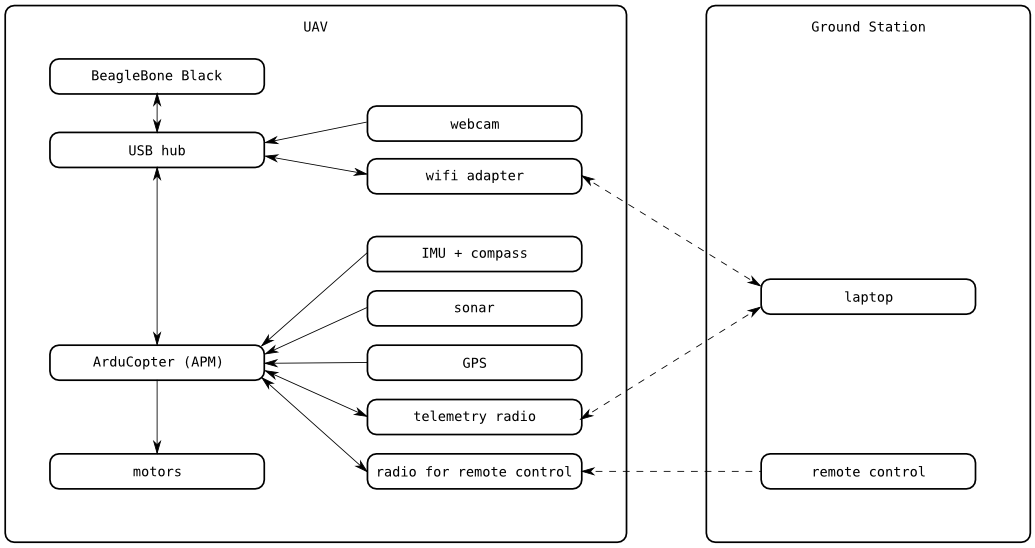
\includegraphics[width=0.9\textwidth]{images/architecture.png}
\caption{
    Architecture of our automated landing system. We use inexpensive
    off-the-shelf hardware. The laptop and remote control are for
    monitoring and emergency takeover by a human pilot. All the
    computation is performed onboard the UAV.
}
\label{fig:hardware-arch}
\end{figure}

\begin{figure}[h!]
\centering
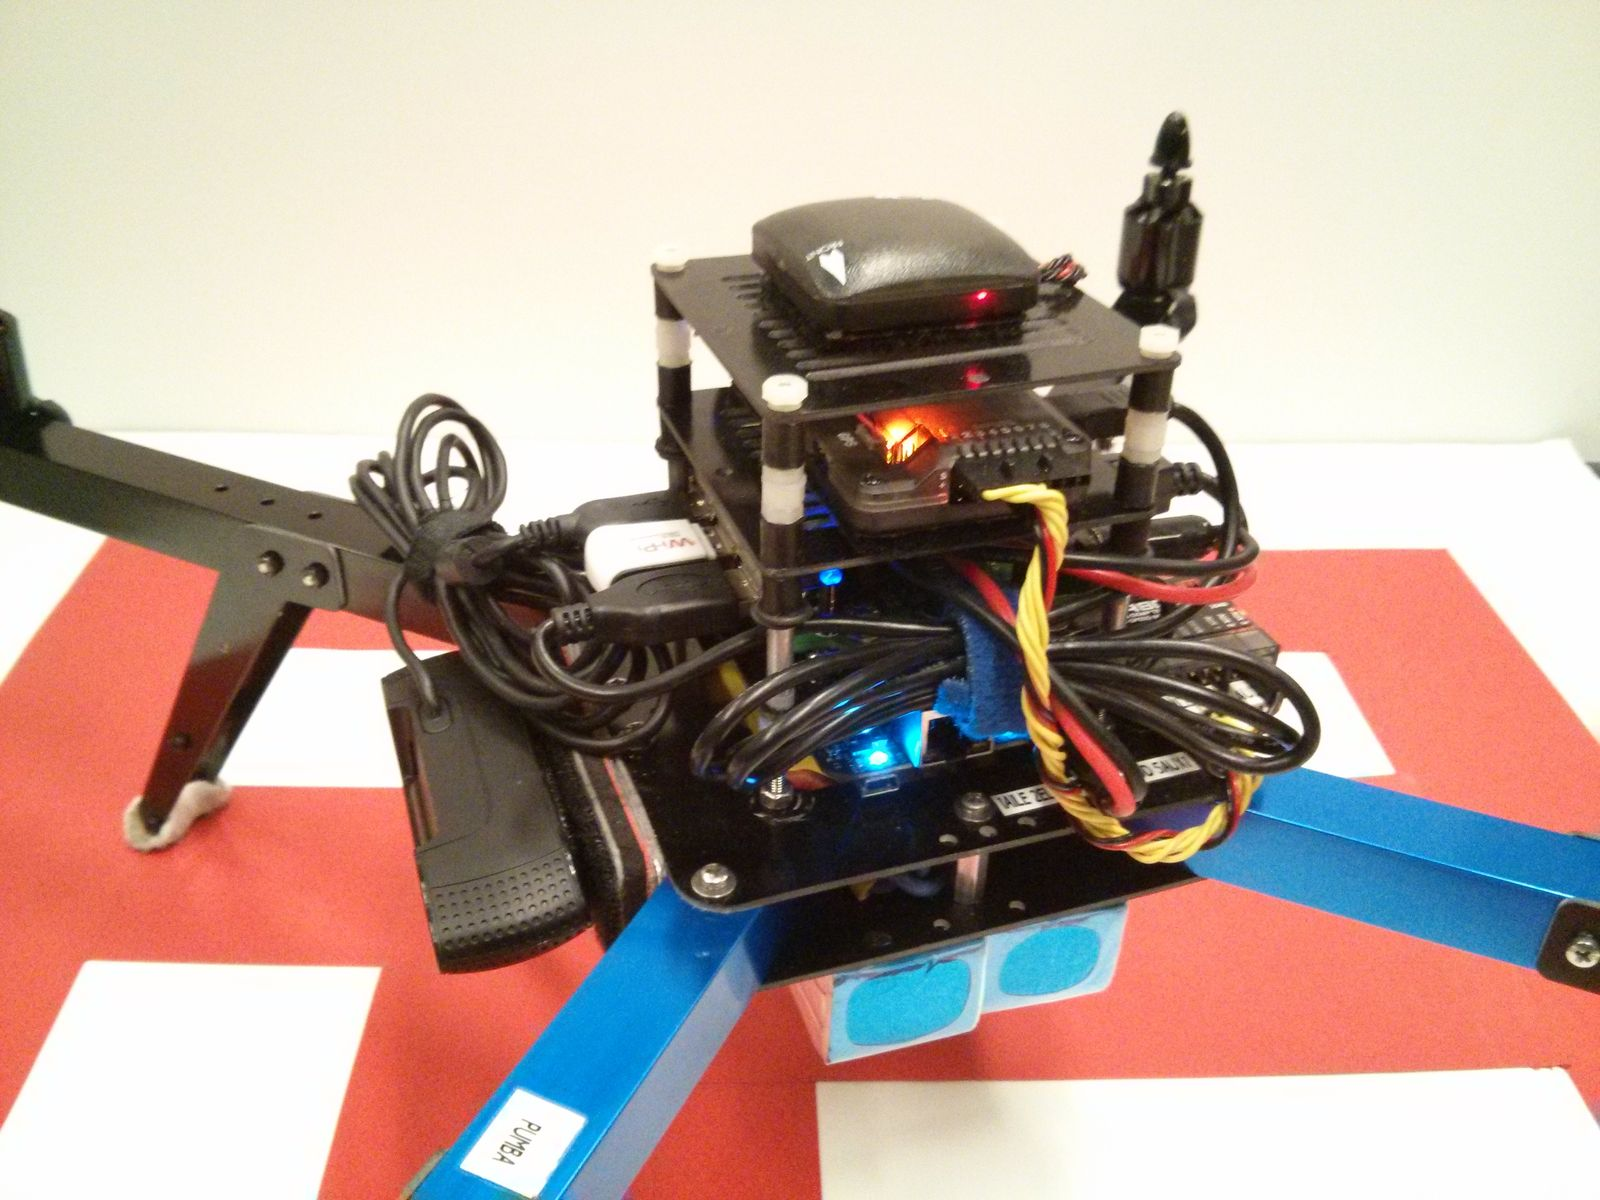
\includegraphics[width=0.85\textwidth]{images/hardware.jpg}
\caption{
    Our hardware stack fully assembled. From bottom to top: batteries,
    BeagleBone embedded computer, USB hub with Wi-Fi adapter, 3D
    Robotics autopilot with embedded sensors, GPS module. The
    webcam is on the left, and the radio for the remote control is on
    the right. Total weight excluding batteries is 1.35 kg.
}
\label{fig:hardware-photo}
\end{figure}

\begin{figure*}[h]
    \centering
    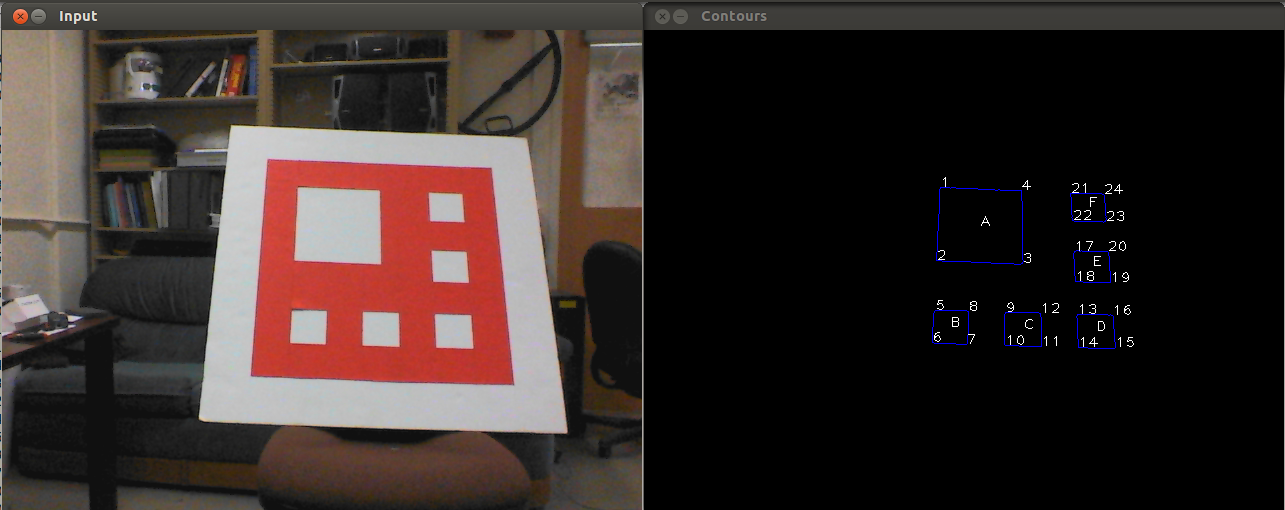
\includegraphics[width=\textwidth]{images/corners.png}
    \caption{
        Left: Design of our landing platform.
        Right: Output of the corner detector (24 points, in order).
    }
    \label{fig:corners}
\end{figure*}

\begin{figure}
    \begin{minipage}{0.5\textwidth}
        \centering
        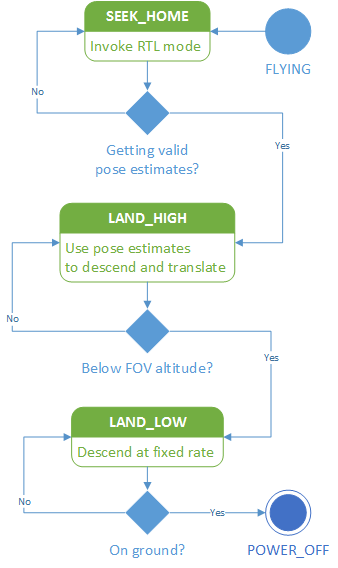
\includegraphics[width=0.9\linewidth]{images/statediagram.png}
        \caption{State diagram of our landing controller.}
        \label{fig:statediagram}
    \end{minipage}% this comment necessary, otherwise extra newline treated as space
    \begin{minipage}{0.5\textwidth}
        \centering
        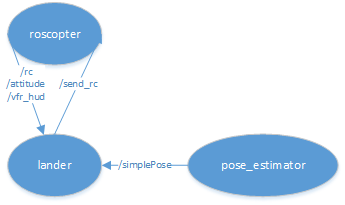
\includegraphics[width=0.9\linewidth]{images/rosnodes.png}
        \caption{ROS nodes and topics for exchanging messages.}
        \label{fig:rosnodes}
        \vspace{2cm}
        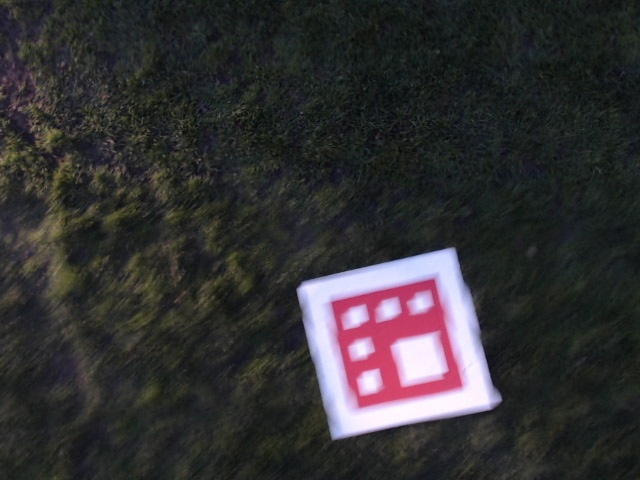
\includegraphics[width=0.9\linewidth]{images/badimage.jpg}
        \caption{An image where pose estimation fails.}
        \label{fig:badimage}
    \end{minipage}
\end{figure}


%
% The following two commands are all you need in the
% initial runs of your .tex file to
% produce the bibliography for the citations in your paper.
%\bibliographystyle{abbrv}
%\bibliography{sigproc}  % sigproc.bib is the name of the Bibliography in this case
\printbibliography
% You must have a proper ".bib" file
%  and remember to run:
% latex bibtex latex latex
% to resolve all references
%
% ACM needs 'a single self-contained file'!
%
%APPENDICES are optional
%\balancecolumns
\appendix
%Appendix A
\end{document}
